% Template:     Archivo de ejemplo
% Versión:      2.0.7 (29/09/2016)
% Codificación: UTF-8
%
% Autor: Pablo Pizarro R.
%        Facultad de Ciencias Físicas y Matemáticas.
%        Universidad de Chile.
%        pablo.pizarro@ing.uchile.cl, ppizarror.com
%
% Licencia: CC BY-NC-SA 4.0 (http://creativecommons.org/licenses/by-nc-sa/4.0/)
% Sitio web del proyecto: http://ppizarror.com/Template-Informe/

% NUEVA SECCIÓN
% Las secciones se inician con \section, si se quiere una sección sin "número" se pueden usar las funciones \newtitleanum (nuevo titulo sin numeración) o la función \newtitleanumnoi para crear el mismo título sin numerar pero sin aparecer en el índice.
\section{Informes con \LaTeX}

	% SUB-SECCIÓN
	% Las sub-secciones se inician con \subsection, si se quiere una sub-sección sin "número" se pueden usar las funciones \newsubtitleanum (nuevo subtitulo sin numeración) o la función \newsubtitleanumnoi para crear el mismo subtítulo sin numerar pero sin aparecer en el índice.
	\subsection{Una breve introducción}
	
		% Esta función sirve para rellenar con un párrafo.
		\lipsum[4]
		
		% Se inserta una ecuación, el primer parámetro entre corchetes es opcional (permite identificar con una etiqueta para poder referenciarlo después con \ref), seguido de aquello se escribe la ecuación en modo bruto sin signos peso.
		\insertequation[\label{eqn:identidad-imposible}]{\pow{a}{k}=\pow{b}{k}+\pow{c}{k}, \forall k>2}
		
		% Los párrafos se pueden añadir con \newpar o simplemente se puede escribir, esta función se hizo para evitar errores y warnings por parte del compilador. Además da la opción de poder cambiar la estructura de todos los párrafos del documento directamente al cambiar las propiedades de la función (definida en la sección DECLARACIÓN DE FUNCIONES).
		\newpar{Este es un párrafo, puede contener múltiples \quotes{Expresiones} así como \quotesit{Citas en itálico} o referencias \footnote{Las referencias se hacen utilizando la expresión \textbackslash label\{etiqueta\}} a fórmulas como (\ref{formulasinsentido}), a continuación se muestra un ejemplo de inserción de imágenes (como la Figura \ref{testimage}):}
		
		% Para insertar una imagen se puede usar la función \insertimage la cual toma un primer parámetro opcional para definir una etiqueta, luego toma la dirección de la imagen, sus parámetros (en este caso se definió la escala de 0.2) y un título de imagen (el cual va debajo de la imagen)
		\insertimage[\label{testimage}]{ejemplos/test-image.png}{scale=0.15}{Where are you? de \quotesit{Internet}}
		
		\newparnl{Este es un párrafo sin nueva linea (de ahí el \textit{nl}, esto se puede usar para terminar un tema, o si vienen imágenes nuevas), si no te gustan los comandos \textbf{newpar} o \textbf{newparnl} simplemente puedes usar los salto de línea convencionales. Además puedes cambiarle el nombre a las funciones, así puedes tener comandos más intuitivos para ti.}
		
	% SUB-SECCIÓN
	\subsection{Tablas!}

		\newparnl{También puedes usar tablas, insertarlas es muy fácil, puedes usar directamente el \quotes{conversor de tablas} \textsuperscript{\cite{conversortabla}}, ahí puedes convertir en un solo clic tablas Excel, o crearlas tú mismo sin tener que hacer todo el aburridísimo código.}
		
		\begin{longtable}{ccc}
			\caption{Esta es una tabla que se \quotes{corta} en varias páginas si es que le falta espacio.}\label{foo}\\
			\hline
			Columna 1 & Columna 2 & Columna 3\\\hline
			\endfirsthead
			\hline
			Columna 1 & Columna 2 & Columna 3\\
			\hline
			\endhead
			\hline
			\endfoot
			\hline
			\endlastfoot
			$\omega$ & $\nu$ & $\delta$\\     
			$\partial$ & $\nabla$ & $\mho$\\
			$\beta$ & $\gamma$ & $\epsilon$\\   
			$\varepsilon$ & $\upsilon$ & $\varphi$\\
			$\Phi$ & $\Theta$ & $\varSigma$\\
			$\omega$ & $\nu$ & $\delta$\\     
			$\partial$ & $\nabla$ & $\mho$\\ 
		\end{longtable}
		
% NUEVA SECCIÓN
\section{Aquí un nuevo tema}
		
	% SUB-SECCIÓN
	\subsection{Haciendo informes como un profesional}
	
		% Se inserta una imagen fija en la izquierda del documento con \insertimageleft, al igual que las demás funciones, el primer parámetro es opcional, luego viene la ubicación de la imagen, seguido de la escala, un título y por último el número de líneas que 'cortará' hacia abajo. Para insertar una imagen fija en la derecha se utiliza \insertimageright usando los mismos parámetros.
		\insertimageleft[\label{imagen-izquierda}]{ejemplos/test-image-wrap}{0.22}{Apolo}{14}
		
		Test es una palabra inglesa aceptada por la Real Academia Española (RAE). Este concepto hace referencia a las pruebas destinadas a evaluar conocimientos, aptitudes o funciones. La palabra test puede utilizarse como sinónimo de examen. Los exámenes son muy frecuentes en el ámbito educativo ya que permiten evaluar los conocimientos adquiridos por los estudiantes. Los exámenes pueden ser orales o escritos, con preguntas de respuestas abiertas (donde el estudiante responde libremente) o preguntas de respuestas múltiples (el estudiante debe seleccionar la respuesta correcta de un listado).
		
		% Se inserta un nuevo párrafo de modo inteligente, evita errores de hbox, crea un nuevo par e espacia de manera fija
		\newp \lipsum[144]
		
		\insertequationcaptioned[\label{formulasinsentido}]{\int_{a}^{b} f(x) dx = \fracnpartial{f(x)}{x}{\eta} \cdotp \textstyle \sum_{x=a}^{b} f(x)\cancelto{1+\frac{\epsilon}{k}}{(1+\Delta x)}}{Ecuación sin sentido}
		
		\begin{wrapfigure}[15]{r}{0.4\textwidth}
			\setcaptionmargincm{0}
			\vspace{-1.0cm}
			\begin{center}
				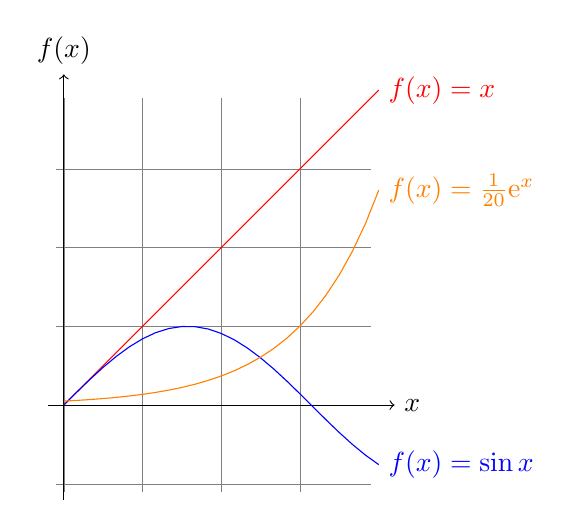
\begin{tikzpicture}[domain=0:4] 
					\draw[very thin,color=gray] (-0.1,-1.1) grid (3.9,3.9);
					\draw[->] (-0.2,0) -- (4.2,0) node[right] {$x$}; 
					\draw[->] (0,-1.2) -- (0,4.2) node[above] {$f(x)$};
					\draw[color=red]    plot (\x,\x)             node[right] {$f(x) =x$}; 
					\draw[color=blue]   plot (\x,{sin(\x r)})    node[right] {$f(x) = \sin x$}; 
					\draw[color=orange] plot (\x,{0.05*exp(\x)}) node[right] {$f(x) = \frac{1}{20} \mathrm e^x$};
				 \end{tikzpicture}
			\end{center}
			\caption{También puedes graficar con \LaTeX !}
			\setcaptionmargincm{\defaultcaptionmargin}
		\end{wrapfigure}
		
		\lipsum[115]
		\vspace{\defaultnewlinesize}
		\lipsum[114]

% REFERENCIAS
\newpage
\begin{thebibliography}{99}
	\addcontentsline{toc}{section}{Referencias}
	
	\bibitem{referencia1} 
		\hbadness=10000 Autor 1, Autor 2.
		\textit{Título}.
		Editorial, versión(revisión):página1:página2, año.
		\\\url{https://www.enlace.com/}
		
	\bibitem{einstein}
		\hbadness=10000 El mismísimo Albert Einstein. 
		\textit{Otro titulo complicado e interesante}. 
		Análisis de físicas de informes, 322(10):891–921, 1905.
	
	\bibitem{pjd} 
		\hbadness=10000 Pedro, Juan y Diego. 
		\textit{Como hacer informes en \LaTeX}. 
		Universidad de Chile, Facultad de Ciencias Físicas y Matemáticas, 2016.
	
	\bibitem{conversortabla}
		\hbadness=10000 Tables Generator.
		\textit{Convierte fácilmente tus tablas, o crea unas con un intuitivo editor de tablas.}
		\\\url{http://www.tablesgenerator.com/}
	
\end{thebibliography}